%%
\documentclass[%
]{ittmm}


% \usepackage[T1]{fontenc}% T2A for Cyrillic font encoding
% \usepackage[english, russian]{babel}

%%% One can fix some overfulls
\sloppy

%% Minted listings support
%% Need pygment <http://pygments.org/> <http://pypi.python.org/pypi/Pygments>
\usepackage{minted}
%% auto break lines
\setminted{breaklines=true}

%% end of the preamble, start of the body of the document source.
\begin{document}

%%
%% Rights management information.
%% CC-BY is default license.
\copyrightyear{2025}
\copyrightclause{Copyright for this paper by its authors.
  Use permitted under Creative Commons License Attribution 4.0
  International (CC BY 4.0).}

%%
%% This command is for the conference information
\conference{Information and Telecommunication Technologies and Mathematical Modeling of High-Tech Systems 2025 (ITTMM 2025), Moscow, April 07--11, 2025}

%%
%% The "title" command
\title{Application of Neural Network Approach to Numerical Integration}

% \tnotemark[1]
% \tnotetext[1]{You can use this document as the template for preparing your publication. We recommend using the latest version of the ittmm style.}

%%
%% The "author" command and its associated commands are used to define
%% the authors and their affiliations.
\author[1]{Gregory Alexandrovich Shipunov}[%
orcid=0009-0007-7819-641X,
email=shgregory3@gmail.com,
]
\cormark[1]

\author[2]{Oksana Ivanovna Streltsova}[%
orcid=0000-0003-4522-6735,
email=!!!,
]

\author[2]{Yuriy Leonidovich Kalinovskiy}[%
orcid=!!!,
email=!!!,
]
\address[1]{Dubna State University,
  19 Universitetskaya St, Dubna, 141980, Russian Federation}
\address[2]{Joint Institute for Nuclear Research,
  6 Joliot-Curie St, Dubna, 141980, Russian Federation}

%%% Footnotes
\cortext[1]{Corresponding author.}

%%
%% The abstract is a short summary of the work to be presented in the
%% article.
\begin{abstract}
    This paper is dedicated to the description of the application of neural network approach to numerical integration of functions of one and multiple variables. The essence of the approach is to train a neural network model to approximate the integral function and than use the parameters of the model to numerically calculate the value of the integral using the formulae based on those parameters. The usage of the approach will reduce the amount of calculations (and time) required to get a numerical integration result when the number of integral function's variables is big. Where the common numerical methods become too complex the numerical approach allows calculations to be less demanding of the computational time and resources. This approach is being tested within the framework of a physics problem of modeling of the particles formation and their properties in the NICA experiment. In this experiment the key problem is to calculate integrals of functions of multiple variables. Currently the author of this paper is developing the framework for integration of functions of two variables. The main goal of the project though is to develop a Python library for numerical integration based on neural network approach.

\end{abstract}

%%
%% Keywords. The author(s) should pick words that accurately describe
%% the work being presented. Separate the keywords with commas.
\begin{keywords}
  neural networks \sep
  numerical integration \sep
  meson \sep
  NICA \sep
  python library
\end{keywords}

%% This command processes the author and affiliation and title
%% information and builds the first part of the formatted document.
\maketitle

\section{Introduction}

The problem of numerical integration appears in both theoretical and applied calculations and potentially raises two obstacles. The first is the complexity of the analytical form of the anti-derivative of the integral function (which is required to get the value of the definite integral). Sometimes it is just hard to produce the anti-derivative of the function and sometimes there are none. In general case there is no general algorithm to get a given function's anti-derivative. Methods of numerical integration exist (e.g. Simpson's method) to solve this problem by providing a formulae to get the value of an integral with some error. But when the number of the integral function's variables grow the complexity of those methods also grows as well as the errors. In this case the neural network approach to the numerical integration may help reduce the complexity as well as increase accuracy of the calculation.

Currently, there were several works done in the field of application of neural networks to the numerical integration problem. We here will highlight the paper "Using neural networks for fast numerical integration and optimization" by Lloyd et al.\cite{lloyd2020using}. This work was served as a source to the development of the neural network approach. Another source was the physics problem of modeling of the particles formation and their properties in the NICA experiment which involves solving the equations containing integrals of 7-dimensional, 10-dimensional and even higher-dimensional integrals. The development of this neural network approach to the numerical integration has the main goal of the development of a Python programming language software library with functionality of numerical integration with usage of neural networks approach.

This paper contains several parts. Firstly, we will give the description of the neural network approach to the numerical integration. Secondly, the physics problem of modeling of the of the particles formation and their properties in the NICA experiment will be depicted. Thirdly, we will give the observation on the results already reached in the development of the neural network approach to the numerical integration. Lastly, the insight on the future of this project will be given. 

\section{Neural Network Approach to Numerical Integration}

The theory of the neural network approach can be summed in the following key points:

\begin{enumerate}
    \item Let 
        \begin{equation}
            I(f) = \int_G f(x)dx,
        \end{equation}
        be a numerical integral of a given function $ f(x) $ across region $G$.
    \item $ f(x) $ can be approximated using a MLP (multi-layer perceptron) neural network $ \hat{f}(x) $.
    \item $ \hat{f}(x) $ can be trained to approximate $ f(x) $ with an arbitrary $ \epsilon $ error bound.
    \item The mathematical form of $ \hat{f}(x) $ can be integrated across given boundaries to produce $\hat{I}(f)$ -- the value of the integral, with the following form (this from is derived from the Lloyd's et al. work\cite{lloyd2020using}):
        \begin{equation}
        \label{eq:numerical_method_1}
            \hat{I}(f) = b^{(2)}\prod_{i=1}^{n}(\beta_i - \alpha_i) + \sum_{j=1}^{k}w_j^{(2)}[\prod_{i=1}^{n}(\beta_i - \alpha_i) + \frac{\Phi_j}{\prod_{i=1}^{n}w_{ij}^{(1)}}],
        \end{equation}
        \begin{equation}
        \label{eq:numerical_method_2}
            \Phi_j = \sum_{r=1}^{2^n}\xi_{r}Li_n(-exp[-b_j^{(1)} - \sum_{i=1}^{n}w_{ij}^{(1)}l_{i,r}]),
        \end{equation}
        \begin{equation}
        \label{eq:numerical_method_3}
            \xi_{r} = \prod_{d=1}^{n}(-1)^{[{r}/{2^{n-d}}]},
        \end{equation}
        \begin{equation}
        \label{eq:numerical_method_4}
            l_{i,r} = \left\{
            \begin{array}{ll}
                \alpha_i, & \text{if } [{r}/{2^{n-d}}] \% 2 = 0 \\
                \beta_i, & \text{if } [{r}/{2^{n-d}}] \% 2 \neq 0,
            \end{array}
        \right.
        \end{equation}
    where $b^{(1)}, b^{(2)}, w^{(1)}, w^{(2)}$ -- neural network's parameters, $\alpha_i, \beta_i, 1 \leq i \leq n$ -- integration boundaries, $n$ -- number of $ f(x) $ variables.
    \item The $\hat{I}(f)$ value can be interpreted as a value of the given numerical integral with an integration error bound $\varepsilon$.
\end{enumerate}

The said MLP architecture should be described in details. The MLP neural network is a simple yet efficient neural network, which contains of several generally 1-dimensional layers $l_i$. Each of the layers contain 1 or many neurons and each neuron form $l_i$ is connected to the each neuron of the $l_{i+1}$ layer. Each neuron value can be changed using an activation function, which modifies the forward-propagated value of the neuron. 

In our case the MLP architecture has 3 layers. The first, input layer, contains of $n$ neurons, where $n$ is the number of integral function variables. The second, hidden layer, contains of $k$ neurons, where $k$ is an arbitrary number greatly influenced by the neural network optimization process. This is the only layer which contains an activation function. The function is a logistic sigmoid function with the form:

\begin{equation}
\label{eq:sigmoid}
    \phi(z) = \frac{1}{1+\exp(-z)}.
\end{equation}

\noindent The third, output layer, contains only one neuron where the $\hat{f}(x)$ value is accumulated. Figure \ref{fig:structure} shows the described architecture.

\begin{figure}
    \centering
    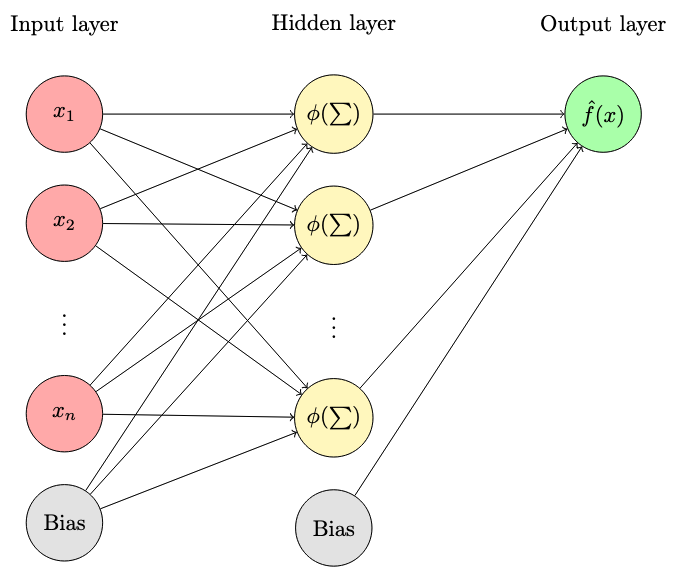
\includegraphics[width=0.6\linewidth]{structure.png}
    \caption{Described MLP structure}
    \label{fig:structure}
\end{figure}

The mathematical form of this MLP structure is:

\begin{equation}
    \label{eq:math-form-mlp}
    \hat{f}(x) = b^{(2)} + \sum_{j=1}^{k}w_j^{(2)}\phi(b_j^{(1)}+\sum_{i=1}^{n}w_{ji}^{(1)}x_{i}),
\end{equation}
where $b^{(1)}, b_j^{(2)}, w_{ji}^{(1)}, w_j^{(2)}$ -- neural network's parameters, $k$ -- number of hidden layer neurons, $n$ -- number of input layer neurons, $\phi$ -- sigmoid function (\ref{eq:sigmoid}).

It is shown in item 3 in the key points of the neural network approach to the numerical integration theory that neural network $\hat{f}(x)$ can be integrated and this operation produces formulae (\ref{eq:numerical_method_1}-\ref{eq:numerical_method_4}). The integration is done quite simply, because mathematical form of the MLP contains of simple arithmetic operation except the sigmoid function. But it also can be integrated simply by substitution:

\begin{equation}
    \label{eq:substitution-li-sigm}
    -Li_0(-\exp(z)) = \frac{1}{1+\exp(-z)} = \phi(z),
\end{equation}

\noindent where $Li_0(u(z))$ is a Jonquière's function or the polylogarithm of order 0:

\begin{equation}
    \label{eq:li0-def}
    Li_0(u) = \frac{u}{1 - u} = -\frac{1}{1 - u^{-1}}.
\end{equation}

With the help of this substitution the integral of the neural network $\hat{f}(x)$ of any number of variables is calculated simply using (\ref{eq:numerical_method_1}-\ref{eq:numerical_method_4}) where, as it can be clearly seen, the polylogarithm is of the same order $n$ as the number of the integration function's variables. (NB: in Python programming language there is mpmath library which contains the required functionality to calculate such an exotic function as the polylogarithm and our numerical integration method also utilizes it.)

To conclude, the neural network approach to numerical integration is:

\begin{enumerate}
    \item generate the dataset to train, validate and test the neural network model (\ref{eq:math-form-mlp}) to approximate given integral function;
    \item train, validate and test (\ref{eq:math-form-mlp}) to approximate given integral function;
    \item extract parameters of the network (\ref{eq:math-form-mlp}) and use them with (\ref{eq:numerical_method_1}-\ref{eq:numerical_method_4}) to calculate the numerical integral.
\end{enumerate}

\section{Physics task}

text

\section{Usage of Neural Network Approach in the Physics task}

text

\section{Future development}

text


%%
%% Define the bibliography file to be used
\bibliography{main}


\end{document}

%%% Local Variables:
%%% mode: LaTeX
%%% TeX-master: t
%%% End:
